\documentclass[aspectratio=169]{beamer}

% Packages
\usepackage[utf8]{inputenc}
\usepackage[english]{babel}
\usepackage{graphicx}
\usepackage{amsmath}
\usepackage{amssymb}
\usepackage{booktabs}
\usepackage{xcolor}
\usepackage{hyperref}

% Theme configurations
\usetheme{Madrid}
\usecolortheme{default}

% Professional Color Palette
\definecolor{navyblue}{RGB}{26, 70, 104}
\definecolor{crimsonred}{RGB}{211, 47, 47}
\definecolor{lightgray}{RGB}{245, 247, 250}

% Apply Colors to Beamer Elements
\setbeamercolor{structure}{fg=navyblue}
\setbeamercolor{palette primary}{bg=navyblue, fg=white}
\setbeamercolor{palette secondary}{bg=navyblue!85, fg=white}
\setbeamercolor{palette tertiary}{bg=navyblue!70, fg=white}
\setbeamercolor{titlelike}{parent=palette primary}
\setbeamercolor{frametitle}{parent=palette primary}
\setbeamercolor{block title}{bg=navyblue, fg=white}
\setbeamercolor{block body}{bg=lightgray, fg=black}

% Remove navigation symbols
\setbeamertemplate{navigation symbols}{}

% Custom footer: hide authors, show only short title, date and frame numbers
\setbeamertemplate{footline}
{
  \leavevmode%
  \hbox{%
  \begin{beamercolorbox}[wd=.666667\paperwidth,ht=2.25ex,dp=1ex,left,leftskip=2ex]{title in head/foot}%
    \usebeamerfont{title in head/foot}\insertshorttitle
  \end{beamercolorbox}%
  \begin{beamercolorbox}[wd=.333333\paperwidth,ht=2.25ex,dp=1ex,right,rightskip=2ex]{date in head/foot}%
    \usebeamerfont{date in head/foot}\insertshortdate{}\hspace*{2em}
    \insertframenumber{} / \inserttotalframenumber
  \end{beamercolorbox}}%
  \vspace{0pt}%
}
% Presenter Information
\title[Offline-First AI for Anemia]{Offline-First Mobile System with AI for the Diagnosis and Prevention of Childhood Anemia in Rural Peru}
\author[Hancco et al.]{Sergio Danilo Hancco Mullisaca \and Eduardo Joel Cuno Salazar \and David Alfredo Huamani Ollachica \and Miguel Angel Alvarez Choque}
\institute[UNSA]{Universidad Nacional de San Agust{\'i}n, Arequipa, Per{\'u}}
\date[July 2026]{Research Presentation -- July 2026}

\begin{document}

% 1. Title Slide
\begin{frame}
    \titlepage
\end{frame}

% 2. Introduction & Context
\begin{frame}{Introduction \& Context}
    \textbf{The Childhood Anemia Crisis in Peru}
    \begin{itemize}
        \item Prevalence of anemia in children aged 6--35 months in rural Peru reaches \textbf{44.7\%} (ENDES).
        \item Traditional diagnosis relies on painful, invasive blood tests, which are unavailable in remote areas.
    \end{itemize}
    \begin{block}{The Vicious Cycle}
        Poor sanitation $\rightarrow$ parasitic infections $\rightarrow$ micro-blood loss $\rightarrow$ chronic anemia.
    \end{block}
    \begin{figure}[H]
        \centering
        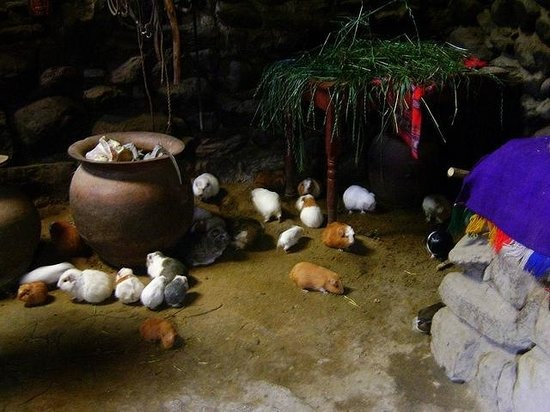
\includegraphics[height=3.0cm]{images/Imagen_De_Prueba_Modulo3.jpeg}
        \caption{Vicious cycle of anemia and sanitational vectors.}
        \label{fig:vicious_cycle_pres}
    \end{figure}
\end{frame}

% 3. Proposed System Architecture
\begin{frame}{Proposed System Architecture}
    \begin{block}{Monorepo Structure (Offline-First and Mesh Sync)}
        An integrated ecosystem designed to work in telecommunication-starved areas with zero infrastructure.
    \end{block}
    \begin{columns}[T]
        \begin{column}{0.48\textwidth}
            \textbf{1. Hybrid Mobile Client (Frontend)}
            \begin{itemize}
                \item Built with \textbf{React Native \& Expo} (Android, iOS).
                \item \texttt{imageProcessor.ts}: Normalizes eyelid images.
                \item \texttt{inferenceEngine.ts}: Local heuristic diagnostic engine.
                \item \texttt{dbService.ts}: SQLite storage for clinical files.
                \item \texttt{gemma\_service.ts}: Environmental vision analyzer.
            \end{itemize}
        \end{column}
        \begin{column}{0.48\textwidth}
            \textbf{2. Central Backend (Node.js/Express)}
            \begin{itemize}
                \item \texttt{sync.controller.ts} (\texttt{/api/sync}): Receives offline data via decentralized mesh nodes.
                \item \texttt{driftDetector.ts} (\texttt{/api/telemetry}): Evaluates accuracy against clinical laboratory results.
                \item \texttt{modelRegistry.ts}: Central version control for active ONNX classifiers.
            \end{itemize}
        \end{column}
    \end{columns}
\end{frame}

% 4. SQLite Relational Database & Local Seeding
\begin{frame}{SQLite Relational Database \& Local Seeding}
    \textbf{Offline Structured Storage managed by \texttt{dbService.ts}}
    \begin{itemize}
        \item \textbf{Entity-Relationship Schema}: Built with SQLite foreign keys enabled (\texttt{PRAGMA foreign\_keys = ON}).
        \item \textbf{Core Relational Tables}:
        \begin{itemize}
            \item \texttt{ecorregiones}: Stores Antonio Brack Egg's 11 geographical regions.
            \item \texttt{alimentos}: Catalog of 15 native Peruvian foods, storing 24 nutritional fields.
            \item \texttt{alimento\_ecorregion}: Many-to-many relationship linking food items to local zones.
            \item \texttt{sustituciones}: Stores equivalency and cost ratios for smart food replacement.
            \item \texttt{historial\_dietas} \& \texttt{diagnosticos}: Relational transactional log tables.
        \end{itemize}
    \end{itemize}
    \begin{block}{Seeded Nutrition Catalog (TPCA-INS)}
        Pre-populated with native Peruvian ingredients (Sangrecita de pollo, Anchoveta, Cuy, Camu Camu, Quinua, Kiwicha, Cañihua, Tarwi, Maca, Sacha Inchi, Aguaymanto, Paiche, etc.) storing macro and micronutrients.
    \end{block}
\end{frame}

% 4. Module 1: Non-Invasive Hemoglobin Estimation
\begin{frame}{Module 1: Non-Invasive Hemoglobin Estimation}
    \textbf{Visual Screening from Palpebral Conjunctiva}
    \begin{enumerate}
        \item \textbf{Image Normalization}: Eyelid photo scaled to $224 \times 224$ pixels.
        \item \textbf{Index Extraction}:
            \begin{itemize}
                \item \textbf{Redness Index ($RI$)}: Evaluates the red pigment level of the mucosal blood vessels.
                \item \textbf{Pallor Index ($PI$)}: Measures average brightness; high values flag pale tissues.
            \end{itemize}
    \end{enumerate}
    
    \begin{block}{Inference \& Physiological Calibration}
        Linear mapping of redness clamped to $RI \in [0.5, 1.8]$ to estimate Base Hemoglobin ($7.5 \text{ to } 13.5 \text{ g/dL}$):
        \begin{equation*}
            Hb_{\text{base}} = 7.5 + (RI_{\text{clamped}} - 0.5) \cdot \frac{13.5 - 7.5}{1.8 - 0.5}
        \end{equation*}
        Adjusted with:
        \begin{itemize}
            \item \textbf{Pallor Penalty}: Deducted if average reflectance exceeds basal thresholds ($PI > 75$).
            \item \textbf{Clinical History Modifier ($M_{\text{hist}}$)}: Compensates according to SQLite records (up to $-1.2$ g/dL if previously Severe).
            \item \textbf{Pediatric Age Adjustments ($F_{\text{edad}}$)}: Factor matching pediatric age groups.
        \end{itemize}
    \end{block}
\end{frame}

% 6. Digital Image Normalization Pipeline
\begin{frame}{Digital Image Normalization Pipeline}
    \textbf{Local Preprocessing pipeline in \texttt{imageProcessor.ts}}
    \begin{columns}[T]
        \begin{column}{0.6\textwidth}
            \begin{itemize}
                \item \textbf{Geometric Resolution Scaling}:
                \begin{itemize}
                    \item Resizes the raw input camera frame to a fixed $224 \times 224$ pixels.
                    \item Handled by \texttt{expo-image-manipulator} to control memory consumption.
                \end{itemize}
                \item \textbf{RGB Chromatic Extraction}:
                \begin{itemize}
                    \item Converts the raw image to base64, sampling colors to find RGB averages.
                \end{itemize}
                \item \textbf{Quantitative Metric Calculations}:
                \begin{itemize}
                    \item \textbf{Redness Index ($RI$)}: Evaluates the intensity of mucosal red.
                    \item \textbf{Pallor Index ($PI$)}: Measures average brightness across channels.
                \end{itemize}
            \end{itemize}
        \end{column}
        \begin{column}{0.38\textwidth}
            \begin{block}{Calculated Indices}
                \begin{equation*}
                    RI = \frac{1}{N} \sum_{i=1}^{N} \frac{R_i}{\frac{G_i + B_i}{2}}
                \end{equation*}
                \begin{equation*}
                    PI = \frac{1}{N} \sum_{i=1}^{N} \frac{R_i + G_i + B_i}{3}
                \end{equation*}
            \end{block}
        \end{column}
    \end{columns}
\end{frame}

% 5. Module 2: Adaptive Nutritional Recommendations
\begin{frame}{Module 2: Adaptive Nutritional Recommendations}
    \textbf{Local Food Database \& Smart Low-Cost Substitution}
    \begin{itemize}
        \item \textbf{Ecorregions Mapping}: 15 native Peruvian foods mapped to Antonio Brack Egg's 11 ecorregions.
        \item \textbf{Substitution Formula}: Replaces expensive meats (e.g. Beef Lomo) with local iron-rich alternatives (Sangrecita).
        \begin{equation*}
            E_g = C_o \cdot \frac{Fe_{\text{original}}}{Fe_{\text{sustituto}}}
        \end{equation*}
        \item \textbf{Impact}: Saves \textbf{85\%} of household costs while increasing bioavailable iron by \textbf{10x}.
    \end{itemize}
    \begin{figure}[H]
        \centering
        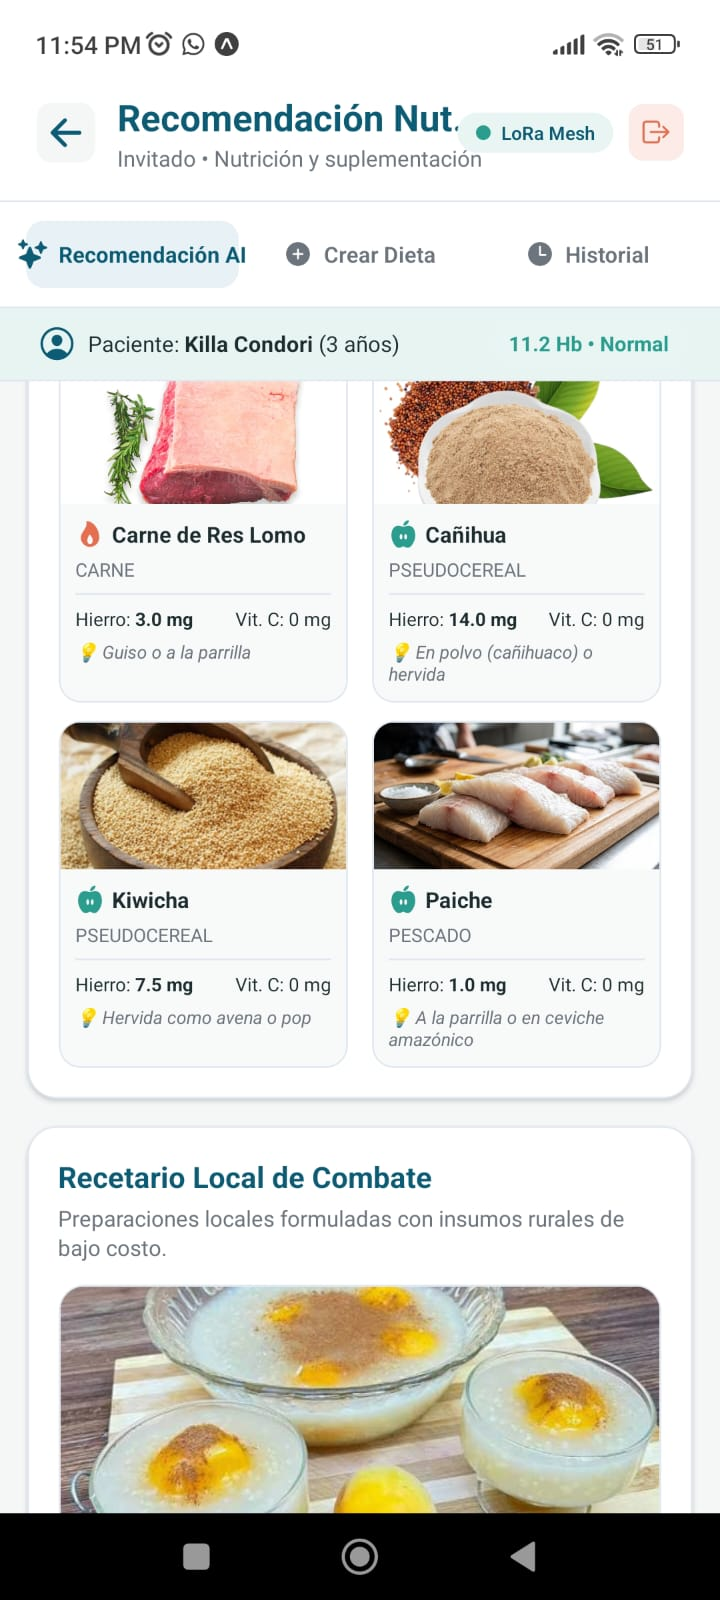
\includegraphics[height=3.0cm]{images/Nutricion.jpeg}
        \caption{Mobile interface for regional recipes.}
        \label{fig:nutricion_pres}
    \end{figure}
\end{frame}

% 6. Module 3: Environmental Prevention via Vision AI
\begin{frame}{Module 3: Environmental Prevention via Vision AI}
    \textbf{Visual Vector Risk Detection with Gemma/LLM Vision}
    \begin{itemize}
        \item Captures environment photos (patios, kitchens) to evaluate vectors (stagnant water, waste).
        \item Generates qualitative risks (Low, Medium, High) and customized hygiene action plans.
    \end{itemize}
    \begin{figure}[H]
        \centering
        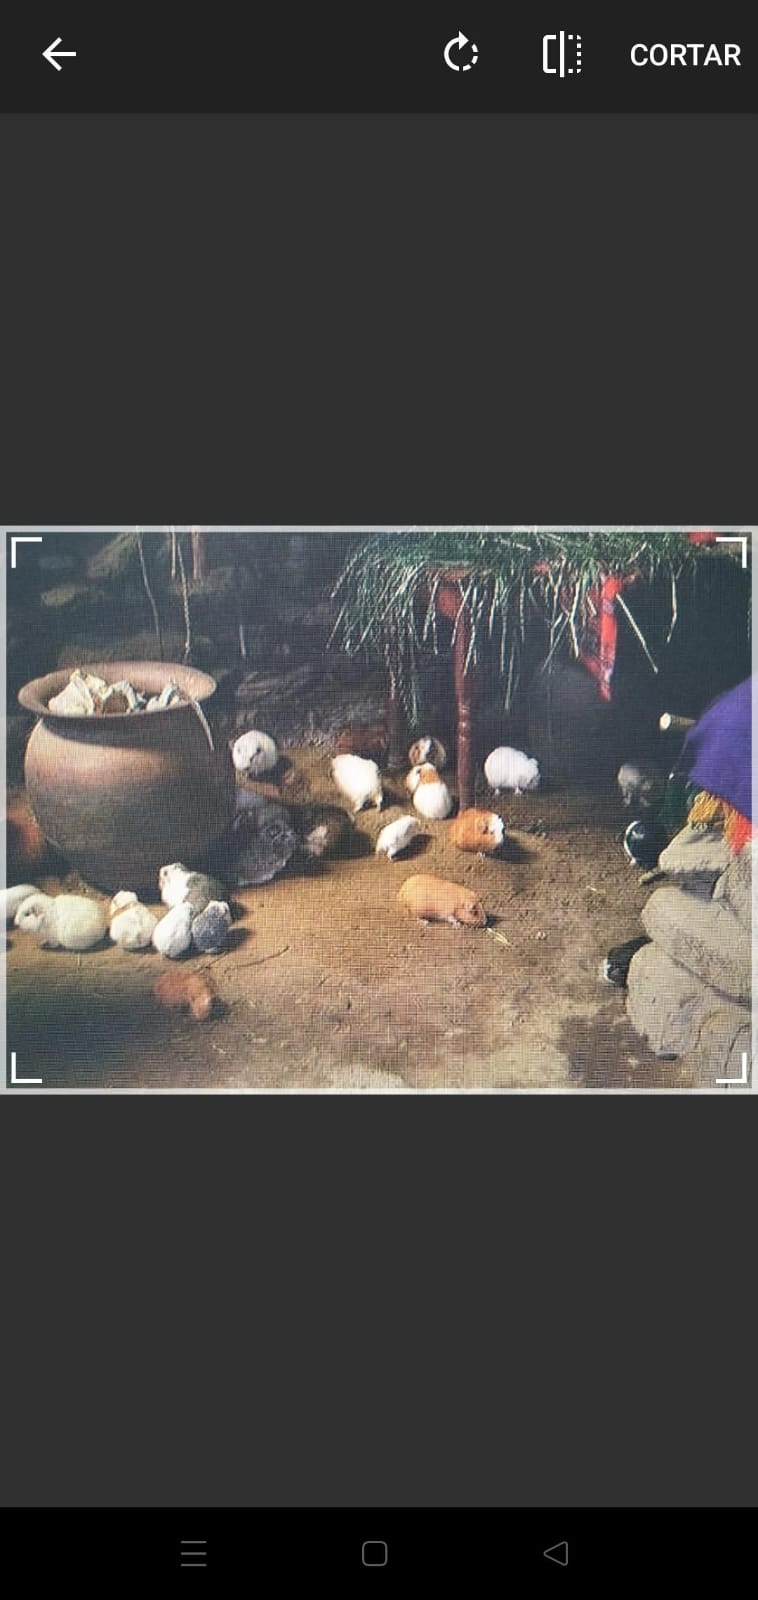
\includegraphics[height=3.0cm]{images/Modulo_Prevencion_Seleccion_Imagen.jpeg}
        \qquad\qquad
        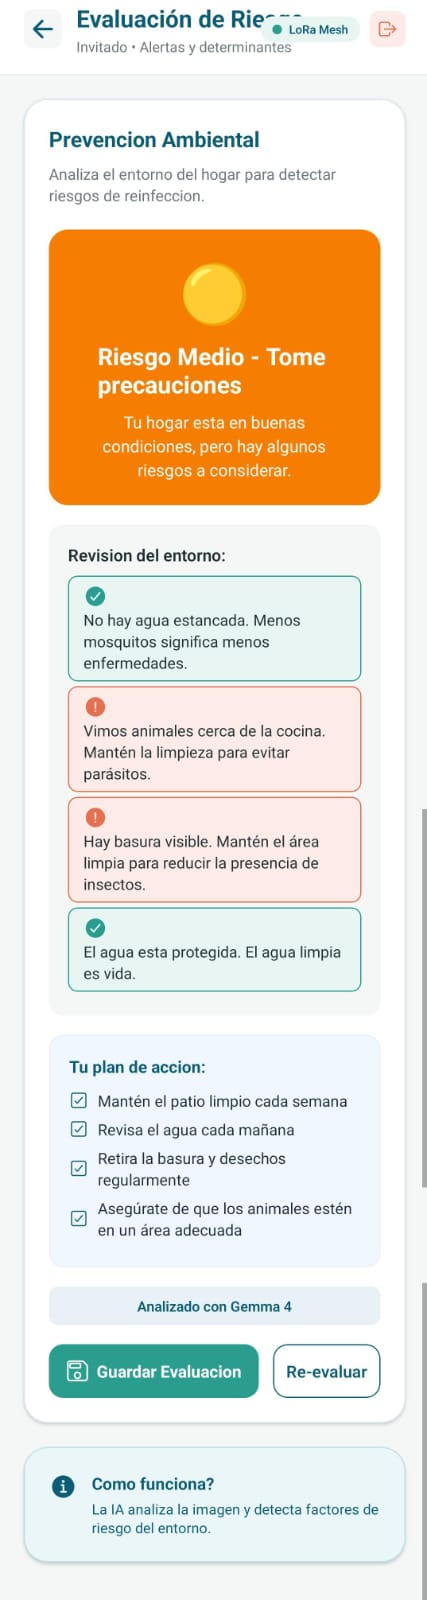
\includegraphics[height=3.0cm]{images/Modulo_Prevencion_Resultado.jpeg}
        \caption{Mobile prevention interface: selection and action plan.}
        \label{fig:prevencion_pres}
    \end{figure}
\end{frame}

% 7. Quantitative Results
\begin{frame}{Quantitative Results}
    \begin{block}{1. Ocular Diagnostic Classifier Performance}
        \begin{itemize}
            \item \textbf{Global Accuracy}: 86.68\% $|$ \textbf{F1 Score (Macro)}: 0.86 $|$ \textbf{MCC}: 0.73
            \item \textbf{Severe Anemia Detection}: F1 Score = 0.91 (critical for immediate clinical referrals).
            \item \textbf{Leve / Normal Ranges}: F1 Score = 0.86 and 0.79 respectively.
        \end{itemize}
    \end{block}
    
    \begin{columns}[T]
        \begin{column}{0.48\textwidth}
            \textbf{2. Nutrition Module Cost Savings}
            \begin{itemize}
                \item \textbf{Yunga region}: 56 food options, cost reduced by \textbf{34\%} (S/ 2.50 average cost).
                \item \textbf{Selva Alta}: 11 local recipes (charqui, paiche), cost reduced by \textbf{41\%} (S/ 2.80 average).
            \end{itemize}
        \end{column}
        \begin{column}{0.48\textwidth}
            \textbf{3. Environmental Risk Detection (LLM)}
            \begin{itemize}
                \item \textbf{Stagnant Water}: F1 = 84.38\% (MCC = 0.71)
                \item \textbf{Open Garbage}: F1 = 85.71\% (MCC = 0.71)
                \item \textbf{Animals near Kitchen}: F1 = 84.38\% (MCC = 0.71)
                \item \textbf{Unprotected Water}: F1 = 88.89\% (MCC = 0.78)
            \end{itemize}
        \end{column}
    \end{columns}
\end{frame}

% 8. Discussion & System Sostenibilidad
\begin{frame}{Discussion \& System Sostenibilidad}
    \begin{columns}[T]
        \begin{column}{0.6\textwidth}
            \textbf{Addressing Anemia Multidimensionally}
            \begin{itemize}
                \item Traditional campaigns fail because child parasitosis causes gut bleeding and blocks iron absorption.
                \item Combining conjunctival screening, local diets, and sanitary checks forms a complete preventive shield.
            \end{itemize}
            \vspace{0.2cm}
            \textbf{Mesh Network Sincronización}
            \begin{itemize}
                \item Offline SQLite logs accumulate on mobile devices during field runs.
                \item Syncs dynamically to the central Node.js backend when a healthcare worker gets close to a local mesh gateway.
            \end{itemize}
        \end{column}
        \begin{column}{0.35\textwidth}
            \begin{block}{Model Drift Telemetry}
                The backend comparisons against blood tests monitor accuracy. If performance drops below \textbf{80\%}, the system triggers a drift warning to recalibrate parameters.
            \end{block}
        \end{column}
    \end{columns}
\end{frame}

% 9. Decentralized LoRa Mesh Synchronization
\begin{frame}{Decentralized LoRa Mesh Synchronization}
    \textbf{Offline-First Data Flow in remote zones}
    \begin{itemize}
        \item \textbf{Local Transactional State}: Diagnoses and custom diets are stored locally with a sync flag (\texttt{sincronizado = 0}).
        \item \textbf{Gateway Proximity Discovery}: Mobile client detects local gateway nodes using mesh networks.
        \item \textbf{Data Sincronización Payload}: Client posts the serialized clinical logs using the \texttt{/api/sync} API.
    \end{itemize}
    \begin{block}{Bidirectional Sync Response}
        The backend registers transaction logs and responds with:
        \begin{itemize}
            \item \textbf{Sincronización Confirmation}: Counts of successfully updated logs.
            \item \textbf{Model Update Alerts}: Returns the \texttt{recommendedModelVersion} (e.g. from \texttt{modelRegistry.ts}) to notify local devices of OTA model updates (e.g., updating the ONNX file).
        \end{itemize}
    \end{block}
\end{frame}

% 10. Model Drift Telemetry & Calibration
\begin{frame}{Model Drift Telemetry \& Calibration}
    \textbf{Continuous Backend Verification in \texttt{driftDetector.ts}}
    \begin{columns}[T]
        \begin{column}{0.55\textwidth}
            \begin{itemize}
                \item \textbf{Real-Time Evaluation}: The backend receives mobile classification outputs compared against gold-standard clinical laboratory blood draws.
                \item \textbf{Performance Tracker}: Computes accuracy, precision, recall, and macro F1 scores in real-time.
                \item \textbf{Drift Alarms}: Activates \texttt{driftDetected = true} if global accuracy drops below the 80\% threshold.
            \end{itemize}
        \end{column}
        \begin{column}{0.4\textwidth}
            \begin{block}{Drift Flag Equation}
                \begin{equation*}
                    \text{Accuracy} = \frac{\sum [P_i == L_i]}{\text{Total Samples}} < 0.80
                \end{equation*}
                Alerts engineering teams to trigger localized model parameters calibration or retrain classes.
            \end{block}
        \end{column}
    \end{columns}
\end{frame}

% 9. Limitations & Future Work
\begin{frame}{Limitations \& Future Work}
    \begin{columns}[T]
        \begin{column}{0.48\textwidth}
            \textbf{Key Limitations}
            \begin{itemize}
                \item \textbf{Optical Noise}: Susceptible to ambient light shifts (direct sun, shadows) and low-end camera sensor distortions.
                \item \textbf{LLM Connectivity}: Visual LLM checks for sanitation vectors depend on the cloud. Fallback mode relies on basic local rules.
                \item \textbf{Cohort Variety}: Requires broader trials to generalize findings to diverse ethnic populations.
            \end{itemize}
        \end{column}
        \begin{column}{0.48\textwidth}
            \textbf{Future Milestones}
            \begin{itemize}
                \item \textbf{On-Device LLMs}: Deploy quantized models (e.g. Gemma 2B) locally via ONNX Runtime Mobile for 100\% offline vision.
                \item \textbf{Physical Color Cards}: Eyelid capture standardizing reference colors to remove ambient light noise.
                \item \textbf{Longitudinal Studies}: Clinical trials (6--12 months) in rural health centers to trace actual recovery rates.
            \end{itemize}
        \end{column}
    \end{columns}
\end{frame}

% 10. Conclusions
\begin{frame}{Conclusions}
    \begin{itemize}
        \item Developed and validated an \textbf{integrated offline-first digital ecosystem} designed specifically for the epidemiology and geographical realities of rural Peru.
        \item Proven clinical feasibility of \textbf{non-invasive hemoglobin screening} (86.68\% accuracy), ensuring immediate detection of life-threatening severe anemia.
        \item Proven economic effectiveness of \textbf{ecorregional food recommendations and substitutions}, reducing diet formulation costs by up to \textbf{41\%} while respecting cultural tastes.
        \item Effective \textbf{prevention checks} via Computer Vision (F1 scores above 84\%), assisting remote communities in breaking the sanitation-parasitosis cycle.
        \item Scalable edge architecture featuring \textbf{LoRa mesh sync and drift telemetry} to secure long-term model calibration and maintenance.
    \end{itemize}
\end{frame}

\end{document}
